\section{OpenStack Foundation}
\frame{
  \frametitle{Características Chave}

  \begin{itemize}
    \item Entidade global e independente
    \item Promover desenvolvimento, distribuição e adoção
    \item Associados
      \begin{itemize}
        \item Indivíduos: gratuito, mas contribuições são esperadas
        \item Empresas: \textit{Platinum}; \textit{Gold}
      \end{itemize}
  \end{itemize}

  \begin{figure}
    \centering
    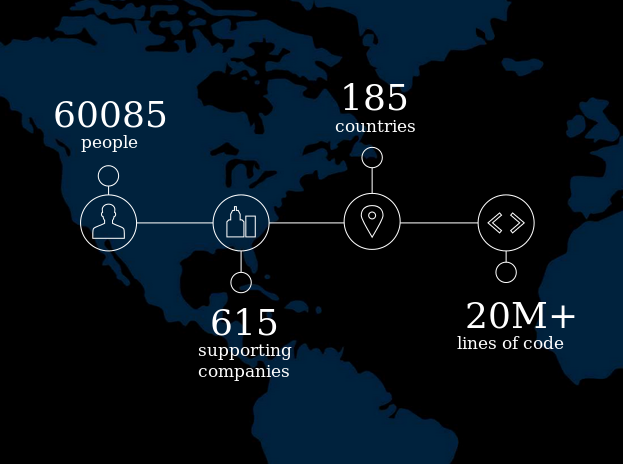
\includegraphics[width=.5\textwidth]{images/global_community.png}
    \caption{Imagem retirada de \url{http://www.openstack.org/} em 05/09/2016}
  \end{figure}
}

\frame{
  \frametitle{Comitê Técnico}
  \begin{columns}
    \begin{column}{.5\textwidth}
      \begin{figure}
        \centering
        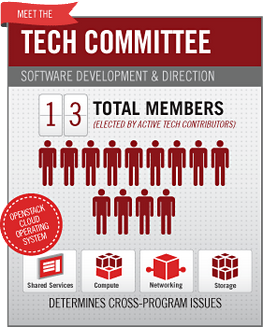
\includegraphics[width=.8\textwidth]{images/tech_comittee.png}
        \caption{Imagem retirada de \url{http://www.openstack.org/foundation/} em 05/09/2016}
      \end{figure}
    \end{column}
    \begin{column}{.5\textwidth}
      \begin{itemize}
        \item Rumo do projeto
        \item Decisões técnicas que afetem múltiplos componentes
      \end{itemize}
    \end{column}
  \end{columns}
}

\frame{
  \frametitle{Corpo de Diretores}

  \begin{columns}
    \begin{column}{.5\textwidth}
      \begin{figure}
        \centering
        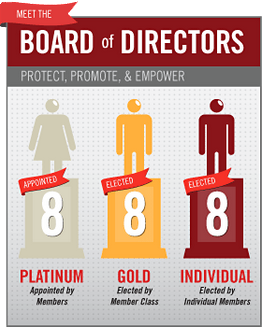
\includegraphics[width=.8\textwidth]{images/board.png}
        \caption{Imagem retirada de \url{http://www.openstack.org/foundation/} em 05/09/2016}
      \end{figure}
    \end{column}
    \begin{column}{.5\textwidth}
      \begin{itemize}
        \item Estratégica
        \item Financeira
      \end{itemize}
    \end{column}
  \end{columns}
}

\frame{
  \frametitle{Comitê de Usuários}

  \begin{columns}
    \begin{column}{.5\textwidth}
      \begin{figure}
        \centering
        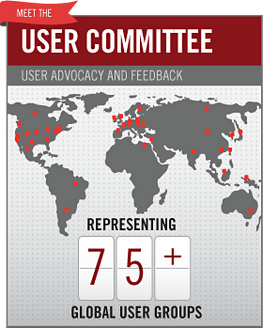
\includegraphics[width=.8\textwidth]{images/user_comittee.png}
        \caption{Imagem retirada de \url{http://www.openstack.org/foundation/} em 05/09/2016}
      \end{figure}
    \end{column}
    \begin{column}{.5\textwidth}
      Criado recentemente para dar representatividade aos grupos globais perante o corpo diretivo e comitê técnico.
    \end{column}
  \end{columns}
}
